\documentclass[40pt,a4paper,UTF8]{ctexart}
\usepackage{amsmath}
\usepackage{graphicx}

\usepackage{float}

%输入带圈数字  eg:\textcircled{1}
\usepackage{fontspec,xunicode-addon}

%代码显示的包
\usepackage{listings}
\usepackage{xcolor}

%打出空心字母
\usepackage{amsfonts,amssymb}

%整体加粗
\usepackage{bm}

%公式按照章节标号
\numberwithin{equation}{section}

%长等号
\usepackage{extpfeil}


%注释用
\usepackage{comment}
%----------------------------------------------
%配置代码显示格式-掌握minted之前的替代品
%----------------------------------------------
\definecolor{codegreen}{rgb}{0,0.6,0}
\definecolor{codegray}{rgb}{0.5,0.5,0.5}
\definecolor{codepurple}{rgb}{0.58,0,0.82}
\definecolor{backcolour}{rgb}{0.95,0.95,0.92}

\lstdefinestyle{mystyle}{
	backgroundcolor=\color{backcolour},   
	commentstyle=\color{codegreen},
	keywordstyle=\color{magenta},
	numberstyle=\tiny\color{codegray},
	stringstyle=\color{codepurple},
	basicstyle=\ttfamily\footnotesize,
	breakatwhitespace=false,         
	breaklines=true,                 
	captionpos=b,                    
	keepspaces=true,                 
	numbers=left,                    
	numbersep=5pt,                  
	showspaces=false,                
	showstringspaces=false,
	showtabs=false,                  
	tabsize=2
}

\lstset{style=mystyle}



%-----------------------------------------------------------------------------------

\title{第七章作业}
\author{Student name: Francisrk}
\date{Due date: March 13th, 2022}

\begin{document}

\maketitle   %控制序列,能将在导言区中定义的标题、作者、日期按照预定的格式展现出来。

\section{第1题}
\paragraph{}
已阅。
\paragraph{}


\section{第2题}
\paragraph{}
\subsection{为何说Bundle Adjustment is slow是不对的?}
文献\cite{ref1}中提到:The claimed slowness is almost always due to the unthinking use of a general-purpose optimization routine that completely ignores
the problem structure and sparseness. Real bundle routines are much more efficient than this, and
usually considerably more efficient and flexible than the newly suggested method.

之前认为BA慢的原因是人们没有意识到问题的结构和稀疏性,直接对H求逆的计算量非常大,也就显得比较慢,但是实际上H具有稀疏性,是可以通过诸如使用Shur消元对H进行Marginalization,从而大大降低计算量,而经过处理之后的BA问题的效率通常比很多新的方法的效率更高,更灵活。

\subsection{BA中有哪些需要注意参数化的地⽅?Pose和Point各有哪些参数化⽅式?有何优缺点。}
\begin{enumerate}
\item 需要参数化的有3D points(路标点y),3D Rotation(相机外参数(R,t)或者说是相机的位姿),相机校准(camera calibration)也就是相机的内参数、投影后的像素坐标。
\item Pose:变换矩阵,欧拉角(Euler Angles),四元数(Quaternions)
\begin{enumerate}
\item 变换矩阵:
优点:旋转轴可以是任意向量
缺点:旋转其实只需要知道一个向量+一个角度(共4自由度),但矩阵却用了16个元素(消耗时间和内存)。

\item 欧拉角:

优点:容易理解,形象直观;三个值分别对应x、y、z轴的旋转角度。

缺点:欧拉角这种方法是要按照一个固定的坐标轴的顺序旋转的,因此不同的顺序会造成不同结果;欧拉角旋转会造成万向锁现象,这种现象的发生就是由于上述固定的坐标轴旋转顺序造成的。由于万向锁的存在,欧拉旋转无法实现球面平滑插值。

\item 四元数:

优点:可以避免万向锁问题;只需要一个4维的四元数就可以执行绕任意过原点的向量的旋转,方便快捷,在某些实现下比旋转矩阵效率更高;而且四元数旋转可以提供平滑插值。

缺点:比欧拉旋转稍微复杂了一点,因为多了一个维度,理解更困难,不直观。带有约束条件。
\end{enumerate}




\item Point:三维坐标点(X,Y,Z),逆深度。

Open VINS文档中给出了五种特征参数化表示:Global XYZ,Global Inverse Depth,Anchored XYZ,Anchored Inverse Depth,Anchored Inverse Depth (MSCKF Version),区别在于:
\begin{enumerate}

\item Global vs Anchored:特征点的表示是全局坐标系的坐标还是局部相机坐标系的坐标。

\item XYZ vs Inverse Depth:使用的XYZ还是逆深度。

\item Two different Inverse Depth:两种不同类型的逆深度参数。

\end{enumerate}
\end{enumerate}

\subsection{*本⽂写于 2000 年,但是⽂中提到的很多内容在后⾯⼗⼏年的研究中得到了印证。你能看到哪些⽅向在后续⼯作中有所体现?请举例说明。}
3.4节的 Intensity- based methods就是BA在直接法中的应用。第5节 Network Structure可以对应到SLAM中的图优化模型;H的稀疏性可以实现BA实时,在07年的PTAM上实现。


\subsection{BAL-dataset}
总结一下BA过程:
\begin{enumerate}
\item 首先选择你想要的图里的节点与边的类型,确定它们的参数化形式;

\item 往图里加入实际的节点和边;

\item 选择初值,开始迭代;

\item 每一步迭代中,计算对应于当前估计值的雅可比矩阵和海塞矩阵;

\item 求解稀疏线性方程$Hk\Delta x=-bk$,得到梯度方向;

\item 继续用GN或LM进行迭代。如果迭代结束,返回优化值。
\end{enumerate}

这里选择了教材上的例程中的数据problem-16-22106-pre.txt文件
核心代码如Listing1所示:

\begin{lstlisting}[language=C++, caption=BAL\_g2o核心代码]
//
// Created by wrk on 2022/3/28.
//

#include <g2o/core/base_vertex.h>
#include <g2o/core/base_binary_edge.h>
#include <g2o/core/block_solver.h>
#include <g2o/core/optimization_algorithm_levenberg.h>
#include <g2o/solvers/csparse/linear_solver_csparse.h>
#include <g2o/core/robust_kernel_impl.h>
#include <iostream>

#include "common.h"
#include "sophus/se3.hpp"

using namespace Sophus;
using namespace Eigen;
using namespace std;

/*
 * 问题梳理:
 * 1.首先,我们需要同时优化相机的位姿和路标点,相机位姿和路标点分别是顶点,
 * 2.然后,误差=观测-预测,采用重投影误差来当做误差
 * 3.最后,将所有的边和顶点插入到图中,构建g2o优化问题求解即可
 * 问题是第二步怎么求重投影?没有深度信息得不到3d点,还是说直接就给了3d的?
 * */

//先定义如何存放姿态,内参,畸变系数
struct PoseAndIntrinsics
{
    PoseAndIntrinsics() {}  //构造函数

    explicit PoseAndIntrinsics(double *data_addr)  //explicit之后只能用()进行初始化,不能用等号进行赋值
    {
        rotation = SO3d::exp(Vector3d(data_addr[0], data_addr[1], data_addr[2]));  //指数映射转换成SO3,罗德里格斯公式
        translation = Vector3d(data_addr[3], data_addr[4], data_addr[5]);
        focal = data_addr[6];
        k1 = data_addr[7];
        k2 = data_addr[8];
    }

    //将估计值放入内存
    void set_to(double *data_addr)
    {
        auto r = rotation.log();   //对数变换得se3
        for(int i=0;i<3;++i) data_addr[i] = r[i];
        for(int i=0;i<3;++i) data_addr[i+3] = translation[i];
        data_addr[6] = focal;
        data_addr[7] = k1;
        data_addr[8] = k2;
    }

    SO3d rotation;  //旋转SO3
    Vector3d translation;  //平移向量
    double focal = 0;  // 焦距
    double k1=0,k2=0;   //畸变系数
};

class VertexPoseAndIntrinsics: public g2o::BaseVertex<9, PoseAndIntrinsics>{
public:
    EIGEN_MAKE_ALIGNED_OPERATOR_NEW;  //重写new,使内存对齐

    VertexPoseAndIntrinsics() {}

    //
    virtual void setToOriginImpl() override
    {
        _estimate = PoseAndIntrinsics();  //这就是要估计的对象:9维数据都需要被估计
    }

    // 估计更新
    virtual void oplusImpl(const double *update) override{
        _estimate.rotation = SO3d::exp(Vector3d(update[0], update[1], update[2])) * _estimate.rotation;
        _estimate.translation += Vector3d(update[3],update[4],update[5]);
        _estimate.focal += update[6];
        _estimate.k1 += update[7];
        _estimate.k2 += update[8];
    }

    //根据估计值投影一个点(估计的是相机系下的3d点)
    Vector2d project(const Vector3d &point){
        Vector3d pc = _estimate.rotation * point + _estimate.translation;
        pc = -pc / pc[2];
        /*
         * 这个畸变的我没看懂
         * */
        double r2 = pc.squaredNorm();
        double distortion = 1.0 + r2 * (_estimate.k1 + _estimate.k2 * r2);
        return Vector2d(_estimate.focal * distortion * pc[0],
                        _estimate.focal * distortion * pc[1]);
    }

    virtual bool read(istream &in) {}

    virtual bool write(ostream &out) const {}
};

class VertexLandMark: public g2o::BaseVertex<3, Eigen::Vector3d>{
public:
    EIGEN_MAKE_ALIGNED_OPERATOR_NEW;  //重写new,使内存对齐

    VertexLandMark() {}

    virtual void setToOriginImpl() override
    {
        _estimate = Eigen::Vector3d(0,0,0);  //这就是要估计的对象:9维数据都需要被估计
    }

    virtual void oplusImpl(const double *update) override{
        _estimate += Eigen::Vector3d(update[0], update[1], update[2]);
    }

    virtual bool read(istream &in) {}

    virtual bool write(ostream &out) const {}
};

//传入参数参数2 :观测值(这里是3D点在像素坐标系下的投影坐标)的维度
//参数Vector :观测值类型,piexl.x,piexl.y
//参数VertexSBAPointXYZ:第一个顶点类型
//参数VertexSE3Expmap :第二个顶点类型
class EdgeProjection: public g2o::BaseBinaryEdge<2, Vector2d, VertexPoseAndIntrinsics, VertexLandMark>{
public:
    EIGEN_MAKE_ALIGNED_OPERATOR_NEW;

//    EdgeProjection(double x): BaseBinaryEdge(),
    virtual void computeError() override  //使用override显式地声明虚函数覆盖
    {
        VertexPoseAndIntrinsics * v0 = dynamic_cast<VertexPoseAndIntrinsics *>(_vertices[0]);  //读取位姿9维顶点
        VertexLandMark * v1 = dynamic_cast<VertexLandMark *>(_vertices[1]);  //读取位姿9维顶点
        // 利用估计的相机位姿和路标点的3d坐标将3d坐标重投影称像素坐标,与观测数据_measurement(实际上就是传进来的Vector2d)计算error,
        // 再由g2o自己计算雅可比,或者我么你自己定义那个2*6的雅可比
        auto proj = v0->project(v1->estimate());
        _error = proj - _measurement;    //为什么不是观测-预测??
    }

    // use numeric derivatives
    virtual bool read(istream &in) {}

    virtual bool write(ostream &out) const {}


};


/*构建g2o问题并求解*/
void SolveBA(BALProblem &bal_problem) {
    const int point_block_size = bal_problem.point_block_size();
    const int camera_block_size = bal_problem.camera_block_size();  //位姿,内参,畸变系数
    double *points = bal_problem.mutable_points();      //  观测点的起始地址
    double *cameras = bal_problem.mutable_cameras();    //  camera参数的起始地址

    // pose dimension 9, landmark is 3
    // 1,2定义blocksolver和linearsolver类型
    typedef g2o::BlockSolver<g2o::BlockSolverTraits<9, 3>> BlockSolverType;
    // 用到对应的LinearSolver就得include对应的.h文件,比如这里的linear_solver_csparse,h
    typedef g2o::LinearSolverCSparse<BlockSolverType::PoseMatrixType> LinearSolverType;
    // 3.选择优化算法,创建总求解器
    auto solver = new g2o::OptimizationAlgorithmLevenberg(
            g2o::make_unique<BlockSolverType>(g2o::make_unique<LinearSolverType>()));
    // 4.创建稀疏优化器
    g2o::SparseOptimizer optimizer;
    optimizer.setAlgorithm(solver);
    optimizer.setVerbose(true);
    // 5.定义图的顶点和边,添加到稀疏优化器中
    const double *observations = bal_problem.observations();  //这个观测值就是前面的4维数据<camera_index_1> <point_index_1> <x_1> <y_1>
    vector<VertexPoseAndIntrinsics *> vertex_pose_intrinsics;  //9维顶点临时变量
    vector<VertexLandMark *> vertex_points;  //3位landmark顶点临时变量
    // 插入相机位姿顶点:3维罗德里格斯旋转向量R,3维平移t,1维焦距f,2维径向畸变系数
    for (int i = 0; i < bal_problem.num_cameras(); ++i) {
        VertexPoseAndIntrinsics *v = new VertexPoseAndIntrinsics();
        double *camera = cameras + camera_block_size * i;
        v->setId(i);
        v->setEstimate(PoseAndIntrinsics(camera));
        optimizer.addVertex(v);
        vertex_pose_intrinsics.push_back(v);
    }
    // 插入路标点(这个)
    for (int i = 0; i < bal_problem.num_points(); ++i)
    {
        VertexLandMark *v = new VertexLandMark();
        double *point = points + point_block_size * i;
        v->setId(i + bal_problem.num_cameras());  //从camera后面开始继续编号
        v->setEstimate(Vector3d(point[0], point[1], point[2]));
        // g2o在BA中需要手动设置待Marg的顶点,在这里设置就是要把路标点给marg掉
        v->setMarginalized(true);
        optimizer.addVertex(v);
        vertex_points.push_back(v);
    }

    //
    for(int i=0; i < bal_problem.num_observations(); ++i)  //观测的数量,2个值算一组观测,所以取值的时候2*i
    {
        EdgeProjection *edge = new EdgeProjection;
        edge->setVertex(0, vertex_pose_intrinsics[bal_problem.camera_index()[i]]);
        edge->setVertex(1, vertex_points[bal_problem.point_index()[i]]);
        edge->setMeasurement(Vector2d(observations[2*i+0], observations[2*i+1]));
        edge->setInformation(Matrix2d::Identity());  //使用单位阵作为协方差矩阵
        edge->setRobustKernel(new g2o::RobustKernelHuber());
        optimizer.addEdge(edge);
    }

    optimizer.initializeOptimization();
    optimizer.optimize(40);

    //优化完成,保存
    //更新相机位姿那9维数据
    for(int i=0; i<bal_problem.num_cameras(); ++i)
    {
        double *camera = cameras + camera_block_size * i;  //找camera地址
        auto vertex = vertex_pose_intrinsics[i];  //取出优化后的9维顶点
        auto estimate = vertex->estimate();  //读取估计值
        estimate.set_to(camera);    //保存至9维顶点
    }
    //更新三维点坐标
    for(int i=0; i<bal_problem.num_points(); ++i)
    {
        double *point = points + point_block_size * i;  //找三维点地址
        auto vertex = vertex_points[i];
        for(int k=0; k<3; ++k)
            point[k] = vertex->estimate()[k];
    }
}


int main(int argc, char** argv)
{
    if (argc != 2) {
        cout << "usage: BAL_g2o bal_data.txt" << endl;
        return 1;
    }
    BALProblem bal_problem(argv[1]);
    bal_problem.Normalize();
    bal_problem.Perturb(0.1, 0.5, 0.5);  //R,t,P标准差,加入噪声
    bal_problem.WriteToPLYFile("initial_g2o.ply");
    SolveBA(bal_problem);
    bal_problem.WriteToPLYFile("final_g2o.ply");
    return 0;
}
\end{lstlisting}

大致使用教材上的例程,加上自己的理解,整理成了博客\cite{ref2}:

选择教材上的数据进行实验,最终运行的结果如图2.1和图2.2所示


\begin{figure}[H]
\centering
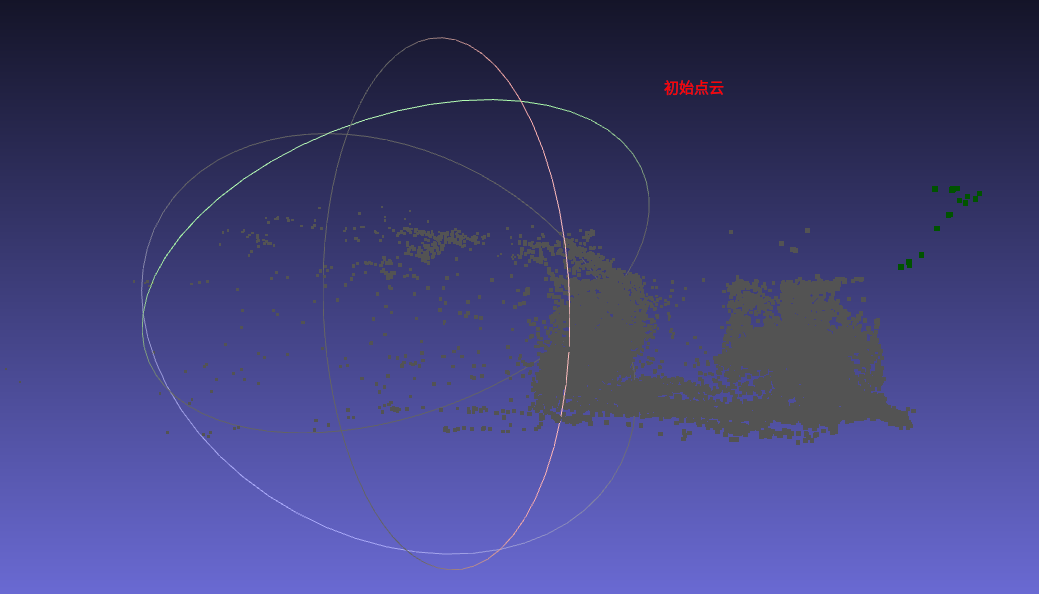
\includegraphics[width=4.8in]{ch7_2_1.jpg} {图2.1 g2o优化前的点云}
\end{figure}

\begin{figure}[H]
\centering
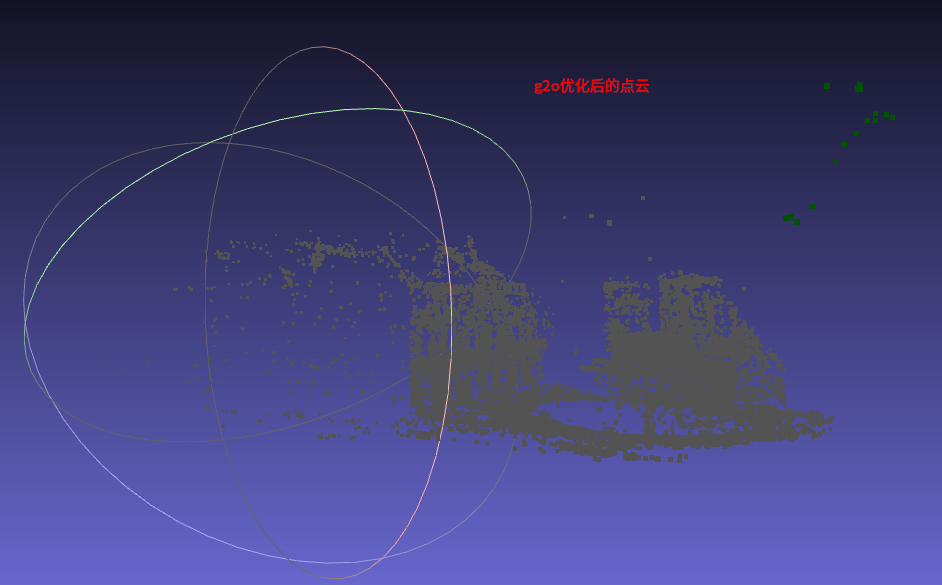
\includegraphics[width=4.8in]{ch7_2_2.jpg} {图2.2 g2o优化后的点云}
\end{figure}

\paragraph{}


\section{直接法的Bundle Adjustment}
\subsection{数学模型}
\begin{enumerate}
\item 如何描述任意⼀点投影在任意⼀图像中形成的 error?
\begin{align}
e = I(\bm p_i)-I_j(\pi(\bm{KT_jp_i}))
\end{align}

\item 每个error关联⼏个优化变量?

每个error关联了2组变量,共9个变量。第1组是相机位姿李代数(6自由度)。第2组是三维路标点位置:$[x,y,z]^T$。

\item error 关于各变量的雅可⽐是什么?

这里的雅可比跟之前的一样,光度误差对路标点的导数是像素梯度*投影方程对相机系下的3d点的导数,见课本P220。

像素梯度:这里采用中心差分进行求导,参照ch6作业
\begin{align}
\frac{\partial \bm I_2}{\partial \bm u}= -\frac{1}{2}
\begin{bmatrix}
I_{2}(u+1,v)-I_{2}(u-1,v) & I_{2}(u,v+1)-I_{2}(u,v-1)
\end{bmatrix}_{1\times 2} \notag \\
\end{align}

投影方程对相机系下的三维点的导数:
\begin{align}
\frac{\partial \bm u}{\partial \bm q}=
\begin{bmatrix}
\frac{f_x}{Z} & 0 & -\frac{f_xX}{Z^2} \\
0 & \frac{f_y}{Z} & -\frac{f_yY}{Z^2}
\end{bmatrix}
\end{align}

相机系下三维点对相机位姿李代数的导数:
\begin{align}
\frac{\partial \bm q}{\partial \delta \bm \xi} &=
\begin{bmatrix}
\bm I, & -\bm q^{\wedge}
\end{bmatrix}
\end{align}
将(3.3)与(3.4)合并得
\begin{align}
\frac{\partial \bm u}{\partial\delta \bm \xi}&=\frac{\partial \bm u}{\partial \bm q}*\frac{\partial \bm q}{\partial \delta \bm \xi} \notag \\
&=
\begin{bmatrix}
\frac{f_x}{Z} & 0 & -\frac{f_xX}{Z^2} & -\frac{f_xXY}{Z^2} & f_x+\frac{f_xX^2}{Z^2} & -\frac{f_xY}{Z} \\
0 & \frac{f_y}{Z} & -\frac{f_yY}{Z^2} & -f_y-\frac{f_yY^2}{Z^2} & \frac{f_yXY}{Z^2} & \frac{f_yX}{Z}
\end{bmatrix}_{2\times 6}
\end{align}

需要说明,因为边连接的是变换之前的路标点P,我们要优化这个路标点的位置,因为q=TP,q是变换之后的3d点,而$\frac{\partial \bm u}{\partial \bm q}$只是对变换之后的3d路标点的导数,为了对变换之前的路标点求导,所以还需要再乘个变换矩阵T。
所以误差对于3d坐标点的雅可比(维数$16\times 3$):
\begin{align}
\bm J_1=-\frac{\partial \bm I_2}{\partial \bm u}\frac{\partial \bm u}{\partial \bm q}  \frac{\partial \bm q}{\partial \bm P} =-\frac{\partial \bm I_2}{\partial \bm u}\frac{\partial \bm u}{\partial \bm q} \bm T
\end{align}
误差对于相机位姿李代数的雅可比(维数$16\times 6$):
\begin{align}
\bm J_2 = \frac{\partial \bm I_2}{\partial \bm u}\frac{\partial \bm u}{\partial  \delta \bm \xi} 
\end{align}
\end{enumerate}

\subsection{实现}
\begin{enumerate}
\item 能否不要以 $[x, y, z]^T$ 的形式参数化每个点?

可以,还可以使用逆深度的方法来参数化每个点,这种方式可以表示无限远点。

\item 取4x4 的patch 好吗?取更⼤的patch 好还是取⼩⼀点的patch 好?

4*4的patch应该是一个比较适中的大小,patch过大会导致计算量大,过小则会导致鲁棒性不强。

\item 从本题中,你看到直接法与特征点法在BA阶段有何不同?

最大的不同是误差定义的不同,而误差又关联着优化的变量,所以优化变量也不同。

直接法是计算光度误差,同时优化相机位姿和3d路标点(如果使用了带深度的3d点,如教材P221上所述,就不用优化路标点了,不知道我这个理解对不对,如果后面看到这里请再思考!)

而特征点法的误差则是重投影误差,只优化相机位姿,因为路标点已经匹配完成。

\item 由于图像的差异,你可能需要鲁棒核函数,例如Huber。此时Huber 的阈值如何选取?

Huber阈值应该是根据多次实验,按照经验来确定的。
\end{enumerate}

代码部分如Listing2所示
\begin{lstlisting}[language=C++, caption=Direct\_BA.cpp]
//
// Created by xiang on 1/4/18.
// this program shows how to perform direct bundle adjustment
//
#include <iostream>

#include <g2o/core/base_unary_edge.h>
#include <g2o/core/base_binary_edge.h>
#include <g2o/core/base_vertex.h>
#include <g2o/core/block_solver.h>
#include <g2o/core/optimization_algorithm_levenberg.h>
#include <g2o/solvers/dense/linear_solver_dense.h>
#include <g2o/core/robust_kernel.h>
#include <g2o/core/robust_kernel_impl.h>
#include <g2o/types/sba/types_six_dof_expmap.h>

#include <Eigen/Core>
#include <sophus/se3.hpp>
#include <opencv2/opencv.hpp>

#include <pangolin/pangolin.h>
#include <boost/format.hpp>

using namespace std;
using namespace Eigen;

typedef vector<Sophus::SE3d, Eigen::aligned_allocator<Sophus::SE3d>> VecSE3;  //装相机位姿
typedef vector<Eigen::Vector3d, Eigen::aligned_allocator<Eigen::Vector3d>> VecVec3d;   //装3d路标点

// global variables
string pose_file = "./poses.txt";
string points_file = "./points.txt";

// intrinsics
float fx = 277.34;
float fy = 291.402;
float cx = 312.234;
float cy = 239.777;

// bilinear interpolation  双线性插值读取图像的灰度值
inline float GetPixelValue(const cv::Mat &img, float x, float y) {
    uchar *data = &img.data[int(y) * img.step + int(x)];
    float xx = x - floor(x);
    float yy = y - floor(y);
    return float(
            (1 - xx) * (1 - yy) * data[0] +
            xx * (1 - yy) * data[1] +
            (1 - xx) * yy * data[img.step] +
            xx * yy * data[img.step + 1]
    );
}

// g2o vertex that use sophus::SE3 as pose  自定义位姿顶点,数据类型是SE3d
class VertexSophus : public g2o::BaseVertex<6, Sophus::SE3d> {
public:
    EIGEN_MAKE_ALIGNED_OPERATOR_NEW

    VertexSophus() {}

    ~VertexSophus() {}


    virtual void setToOriginImpl() {
        _estimate = Sophus::SE3d();
    }

    //根据估计值投影一个点(估计的是相机系下的3d点)
    Vector2f project(const Vector3d &point)
    {
        //KTP 读取SE(3),转换,投影为像素坐标,访问像素灰度值计算光度误差
        Sophus::SE3d Tcw(estimate());
        Vector3d point_cam3d = Tcw * point;
        float u = fx * point_cam3d[0]/point_cam3d[2] + cx;
        float v = fy * point_cam3d[1]/point_cam3d[2] + cy;
        return Vector2f(u,v);
    }

    //更新
    virtual void oplusImpl(const double *update_) {
        //计算se(3),再由se(3)为SE(3)
        Eigen::Map<const Eigen::Matrix<double, 6, 1>> update(update_);
        //保存估计值,相当于_estimate = Sophus::SE3d::exp(update) * _estimate;
        setEstimate(Sophus::SE3d::exp(update) * estimate());
    }

    virtual bool read(std::istream &is) {}

    virtual bool write(std::ostream &os) const {}
};

// TODO edge of projection error, implement it
// 16x1 error, which is the errors in patch   16个像素点的光度差之和
typedef Eigen::Matrix<double,16,1> Vector16d;
class EdgeDirectProjection : public g2o::BaseBinaryEdge<16, Vector16d, g2o::VertexSBAPointXYZ, VertexSophus>  //一个是SBA的XYZ自带边,一个是自定义的边
        {
public:
    EIGEN_MAKE_ALIGNED_OPERATOR_NEW;

    //边构造函数
    EdgeDirectProjection(float *color, cv::Mat &target) {
        this->origColor = color;
        this->targetImg = target;
    }

    ~EdgeDirectProjection() {}

    virtual void computeError() override {
        // TODO START YOUR CODE HERE
        // compute projection error ...
        //projected = KTP  需要使用SE(3)
        g2o::VertexSBAPointXYZ* vertexPw = static_cast<g2o::VertexSBAPointXYZ *>(_vertices[0]);
        VertexSophus* vertexTcw = static_cast<VertexSophus *>(_vertices[1]);
        Vector2f proj = vertexTcw->project(vertexPw->estimate());
        //判断是否越界,若越界,则将error该位置1,并setLevel(1)不知道啥意思,是记录好坏的吗?
        if(proj[0]<-2 || proj[0]+2>targetImg.cols || proj[1]<-2 || proj[1]+2>targetImg.rows)
        {
            this->setLevel(1);  //设置level为1,标记为outlier,下次不再对该边进行优化
            for(int i=0; i<16; ++i)  _error[i] = 0;  //_error是16*1的向量
        }
        else{
            for(int i=-2; i<2;++i){
                for(int j=-2; j<2; ++j){
                    /*******************************************************/
                    int num = 4 * i + j + 10;   //为什么要加10???????????????????????
                    /*******************************************************/
                    //_measurement是一个16*1的向量,所以_error也是16*1
                    _error[num] = origColor[num] - GetPixelValue(targetImg, proj[0]+i, proj[1]+j);
                }
            }
        }
        // END YOUR CODE HERE
    }
    // Let g2o compute jacobian for you  自己不算了,后面再算
    virtual void linearizeOplus() override
    {

        //分别计算3d点和李代数的雅可比
//        J_I2u
//        J_uq
//        J_qxi
        if(level()==1)
        {
            _jacobianOplusXi = Eigen::Matrix<double, 16, 3>::Zero();  //因为_error是(D,1)的,D=16是4*4的patch,所以对第一个顶点的雅可比就是16*2*2*3=16*3的
            _jacobianOplusXj = Eigen::Matrix<double, 16, 6>::Zero();  //同理,对第二个顶点(李代数顶点)的雅可比是16*2*2*3*3*6=16*6的
            return;
        }

        g2o::VertexSBAPointXYZ *vertexPw = static_cast<g2o::VertexSBAPointXYZ *> (_vertices[0]);
        VertexSophus *vertexTcw = static_cast<VertexSophus *> (_vertices[1]);
        Vector2f proj = vertexTcw->project(vertexPw->estimate());

        double X = vertexPw->estimate()[0], Y = vertexPw->estimate()[1], Z = vertexPw->estimate()[2];
        double inv_z = 1.0 / Z, inv_z2 = inv_z * inv_z;  //cur中的3D坐标X'Y'Z'
        float u = proj[0], v = proj[1];

        Eigen::Matrix<double,1,2> J_I2u;    //像素梯度
        Eigen::Matrix<double,2,3> J_uq;     //投影方程对3d点导数
        Eigen::Matrix<double,3,6> J_qxi = Eigen::Matrix<double,3,6>::Zero();    //3d点对李代数导数

        J_uq(0,0) = fx * inv_z;
        J_uq(0,1) = 0;
        J_uq(0,2) = -(fx*X) * inv_z2;
        J_uq(1,0) = 0;
        J_uq(1,1) = fy * inv_z;
        J_uq(1,2) = -fy * Y * inv_z2;

        //这个矩阵见P187笔记[I| -P'^]
        J_qxi(0,0) = 1;
        J_qxi(0,4) = Z;
        J_qxi(0,5) = -Y;
        J_qxi(1,1) = 1;
        J_qxi(1,3) = -Z;
        J_qxi(1,5) = X;
        J_qxi(2,2) = 1;
        J_qxi(2,3) = -Y;
        J_qxi(2,4) = -X;

        for(int x=-2; x<2; ++x)
            for(int y=-2; y<2; ++y)
            {
                //这num到底是什么意思???实际上是计算patch中第几个,num=4*(x+2)+(y+2)=4x+y+10
                int num = 4 * x + y + 10;

                //中心差分计算像素梯度
                J_I2u(0,0) = (1.0 / 2) * (GetPixelValue(targetImg, u+1+x, v+y)-GetPixelValue(targetImg, u-1+x, v+y));
                J_I2u(0,1) = (1.0 / 2) * (GetPixelValue(targetImg, u+x, v+1+y)-GetPixelValue(targetImg, u+x, v-1+y));

                /********为什么还要乘以一个变换矩阵?******/
//                _jacobianOplusXi.block<1, 3>(num, 0) = -J_I2u * J_uq * vertexTcw->estimate().rotationMatrix();
                _jacobianOplusXi.block<1, 3>(num, 0) = -J_I2u * J_uq ;

                _jacobianOplusXj.block<1, 6>(num, 0) = -J_I2u * J_uq * J_qxi;

            }
    }

    virtual bool read(istream &in) {}

    virtual bool write(ostream &out) const {}

private:
    cv::Mat targetImg;  // the target image
    float *origColor = nullptr;   // 16 floats, the color of this point
};

// plot the poses and points for you, need pangolin
void Draw(const VecSE3 &poses, const VecVec3d &points, string title);

int main(int argc, char **argv) {

    // read poses and points
    VecSE3 poses;
    VecVec3d points;
    ifstream fin(pose_file);  //读取相机位姿(7张图,7个位姿)

    //读取位姿
    while (!fin.eof())
    {
        double timestamp = 0;
        fin >> timestamp;
        if (timestamp == 0) break;
        double data[7];
        for (auto &d: data) fin >> d;
        //四元数和平移向量来构建SE3
        poses.push_back(Sophus::SE3d
        (
                Eigen::Quaterniond(data[6], data[3], data[4], data[5]),
                Eigen::Vector3d(data[0], data[1], data[2])
        ));
        if (!fin.good()) break;
    }
    fin.close();

    //读取3d路标点XYZ
    vector<float *> color;
    fin.open(points_file);
    while (!fin.eof())
    {
        double xyz[3] = {0};
        for (int i = 0; i < 3; i++) fin >> xyz[i];
        if (xyz[0] == 0) break;
        points.push_back(Eigen::Vector3d(xyz[0], xyz[1], xyz[2]));
        float *c = new float[16];
        for (int i = 0; i < 16; i++) fin >> c[i];
        color.push_back(c);

        if (fin.good() == false) break;
    }
    fin.close();

    cout << "poses: " << poses.size() << ", points: " << points.size() << endl;


    // read images 读取所有图片
    vector<cv::Mat> images;
    boost::format fmt("./%d.png");
    for (int i = 0; i < 7; i++)
    {
        images.push_back(cv::imread((fmt % i).str(), 0));
    }

    // build optimization problem
    typedef g2o::BlockSolver<g2o::BlockSolverTraits<6, 3>> DirectBlock;  // 求解的向量是6*1的
    typedef g2o::LinearSolverDense<DirectBlock::PoseMatrixType> LinearSolverType;
//    DirectBlock::LinearSolverType *linearSolver = new g2o::LinearSolverDense<DirectBlock::PoseMatrixType>();
//    DirectBlock *solver_ptr = new DirectBlock(linearSolver);
    auto solver = new g2o::OptimizationAlgorithmLevenberg(g2o::make_unique<DirectBlock>(g2o::make_unique<LinearSolverType>()));
    g2o::SparseOptimizer optimizer;
    optimizer.setAlgorithm(solver);
    optimizer.setVerbose(true);

    // TODO add vertices, edges into the graph optimizer
    vector<g2o::VertexSBAPointXYZ *> vertex_points;  //3位landmark顶点临时变量
    vector<VertexSophus *> vertex_pose;  //pose顶点临时变量

    // START YOUR CODE HERE
    //插入路标顶点
    for(int i=0; i<points.size(); ++i)
    {
        g2o::VertexSBAPointXYZ *v = new g2o::VertexSBAPointXYZ;
        v->setId(i);
        v->setEstimate(points[i]);
        v->setMarginalized(true);   //设置边缘化路标点
        optimizer.addVertex(v);
        vertex_points.push_back(v);
    }
    //插入位姿顶点
    for(int i=0; i<poses.size(); ++i)
    {
        VertexSophus *v = new VertexSophus();
        v->setId(i + points.size());
        v->setEstimate(poses[i]);
        optimizer.addVertex(v);
        vertex_pose.push_back(v);
    }

    //插入边
    for(int c=0; c<poses.size(); ++c)
        for(int p=0; p<points.size(); ++p)
        {
            EdgeDirectProjection *edge = new EdgeDirectProjection(color[p], images[c]);  //每个图中的每个点都插入到优化图中,都有一条边
            //先point后pose
            edge->setVertex(0, dynamic_cast<g2o::VertexSBAPointXYZ *>(optimizer.vertex(p)));
            edge->setVertex(1, dynamic_cast<VertexSophus *>(optimizer.vertex(points.size()+c)));
//            edge->setMeasurement(Vector16d );
            // 信息矩阵可直接设置为 error_dim*error_dim 的单位阵
            edge->setInformation(Eigen::Matrix<double, 16, 16>::Identity());
            // 设置Huber核函数,减小错误点影响,加强鲁棒性
            g2o::RobustKernelHuber *rk = new g2o::RobustKernelHuber;
            rk->setDelta(1.0);  //A squared error above delta^2 is considered as outlier in the data
            edge->setRobustKernel(rk);
            optimizer.addEdge(edge);
        }

    // END YOUR CODE HERE

    Draw(poses, points, string("before"));

    // perform optimization
    optimizer.initializeOptimization(0);
    optimizer.optimize(100);

    // TODO fetch data from the optimizer
    // START YOUR CODE HERE
    for(int c=0; c<poses.size(); ++c)
        for(int p=0; p<points.size(); ++p)
        {
            points[p] = dynamic_cast<g2o::VertexSBAPointXYZ *>(optimizer.vertex(p))->estimate();
            poses[c] = dynamic_cast<VertexSophus *>(optimizer.vertex(points.size()+c))->estimate();
        }

    // END YOUR CODE HERE

    // plot the optimized points and poses
    Draw(poses, points, "after");

    // 看看这数据有没有什么不一样的?怎么看优化的对不对?


    // delete color data
    for (auto &c: color) delete[] c;
    return 0;
}

void Draw(const VecSE3 &poses, const VecVec3d &points, string title) {
    if (poses.empty() || points.empty()) {
        cerr << "parameter is empty!" << endl;
        return;
    }

    // create pangolin window and plot the trajectory
    pangolin::CreateWindowAndBind(title, 1024, 768);
    glEnable(GL_DEPTH_TEST);
    glEnable(GL_BLEND);
    glBlendFunc(GL_SRC_ALPHA, GL_ONE_MINUS_SRC_ALPHA);

    pangolin::OpenGlRenderState s_cam(
            pangolin::ProjectionMatrix(1024, 768, 500, 500, 512, 389, 0.1, 1000),
            pangolin::ModelViewLookAt(0, -0.1, -1.8, 0, 0, 0, 0.0, -1.0, 0.0)
    );

    pangolin::View &d_cam = pangolin::CreateDisplay()
            .SetBounds(0.0, 1.0, pangolin::Attach::Pix(175), 1.0, -1024.0f / 768.0f)
            .SetHandler(new pangolin::Handler3D(s_cam));


    while (pangolin::ShouldQuit() == false) {
        glClear(GL_COLOR_BUFFER_BIT | GL_DEPTH_BUFFER_BIT);

        d_cam.Activate(s_cam);
        glClearColor(0.0f, 0.0f, 0.0f, 0.0f);

        // draw poses
        float sz = 0.1;
        int width = 640, height = 480;
        for (auto &Tcw: poses) {
            glPushMatrix();
            Sophus::Matrix4f m = Tcw.inverse().matrix().cast<float>();
            glMultMatrixf((GLfloat *) m.data());
            glColor3f(1, 0, 0);
            glLineWidth(2);
            glBegin(GL_LINES);
            glVertex3f(0, 0, 0);
            glVertex3f(sz * (0 - cx) / fx, sz * (0 - cy) / fy, sz);
            glVertex3f(0, 0, 0);
            glVertex3f(sz * (0 - cx) / fx, sz * (height - 1 - cy) / fy, sz);
            glVertex3f(0, 0, 0);
            glVertex3f(sz * (width - 1 - cx) / fx, sz * (height - 1 - cy) / fy, sz);
            glVertex3f(0, 0, 0);
            glVertex3f(sz * (width - 1 - cx) / fx, sz * (0 - cy) / fy, sz);
            glVertex3f(sz * (width - 1 - cx) / fx, sz * (0 - cy) / fy, sz);
            glVertex3f(sz * (width - 1 - cx) / fx, sz * (height - 1 - cy) / fy, sz);
            glVertex3f(sz * (width - 1 - cx) / fx, sz * (height - 1 - cy) / fy, sz);
            glVertex3f(sz * (0 - cx) / fx, sz * (height - 1 - cy) / fy, sz);
            glVertex3f(sz * (0 - cx) / fx, sz * (height - 1 - cy) / fy, sz);
            glVertex3f(sz * (0 - cx) / fx, sz * (0 - cy) / fy, sz);
            glVertex3f(sz * (0 - cx) / fx, sz * (0 - cy) / fy, sz);
            glVertex3f(sz * (width - 1 - cx) / fx, sz * (0 - cy) / fy, sz);
            glEnd();
            glPopMatrix();
        }

        // points
        glPointSize(2);
        glBegin(GL_POINTS);
        for (size_t i = 0; i < points.size(); i++) {
            glColor3f(0.0, points[i][2]/4, 1.0-points[i][2]/4);
            glVertex3d(points[i][0], points[i][1], points[i][2]);
        }
        glEnd();

        pangolin::FinishFrame();
        usleep(5000);   // sleep 5 ms
    }
}
\end{lstlisting}

优化前的点云图如图3.1所示,优化后的如图3.2所示
\begin{figure}[H]
\centering
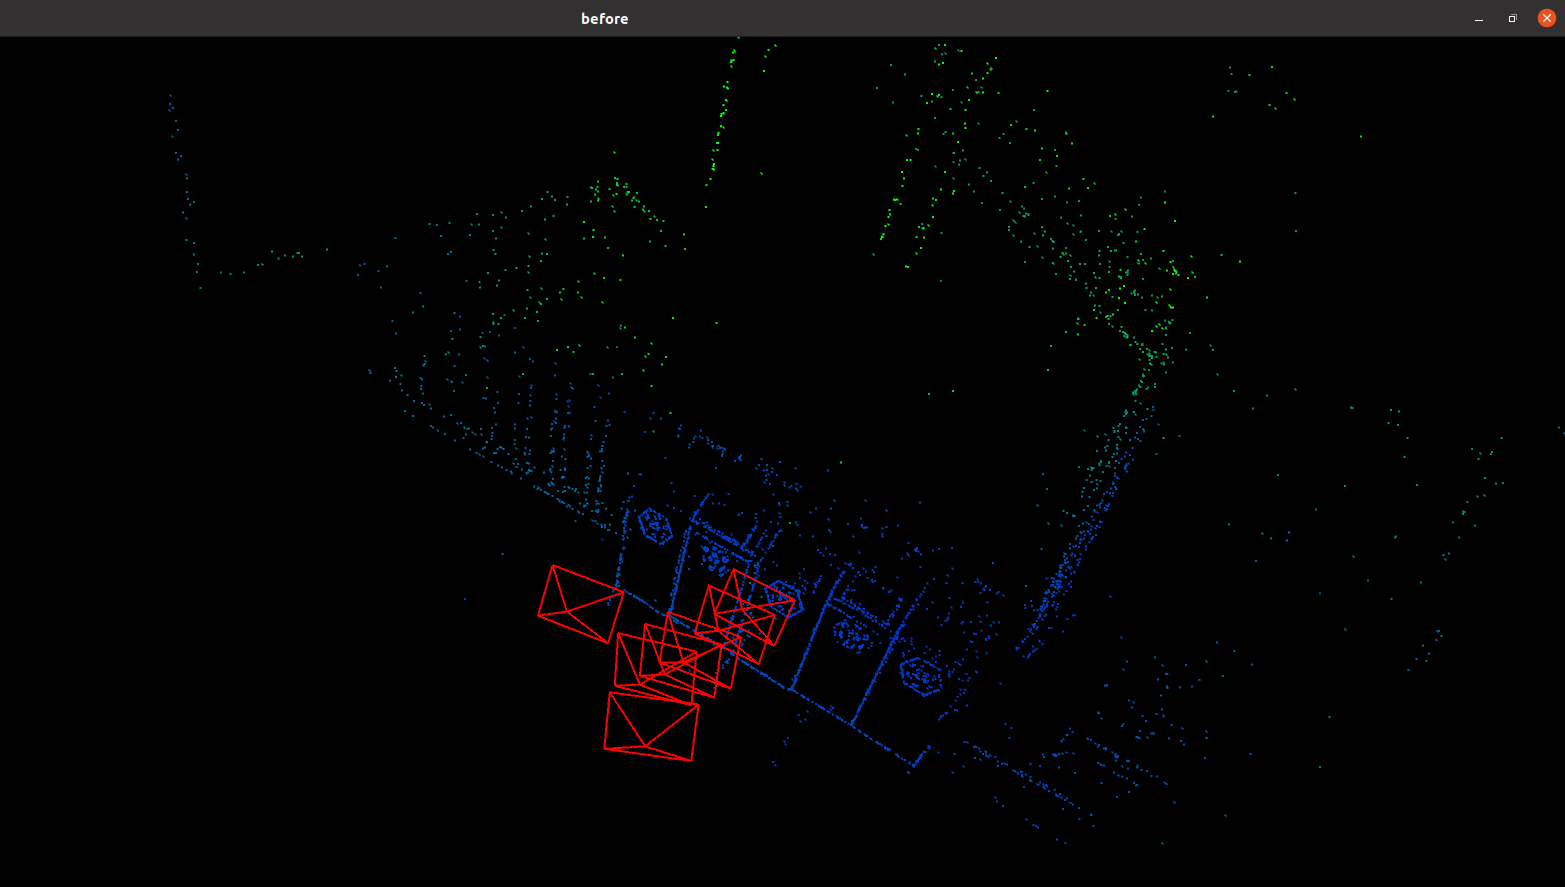
\includegraphics[width=4.8in]{ch7_3_1.png} {图3.1 g2o优化前的点云}
\end{figure}

\begin{figure}[H]
\centering
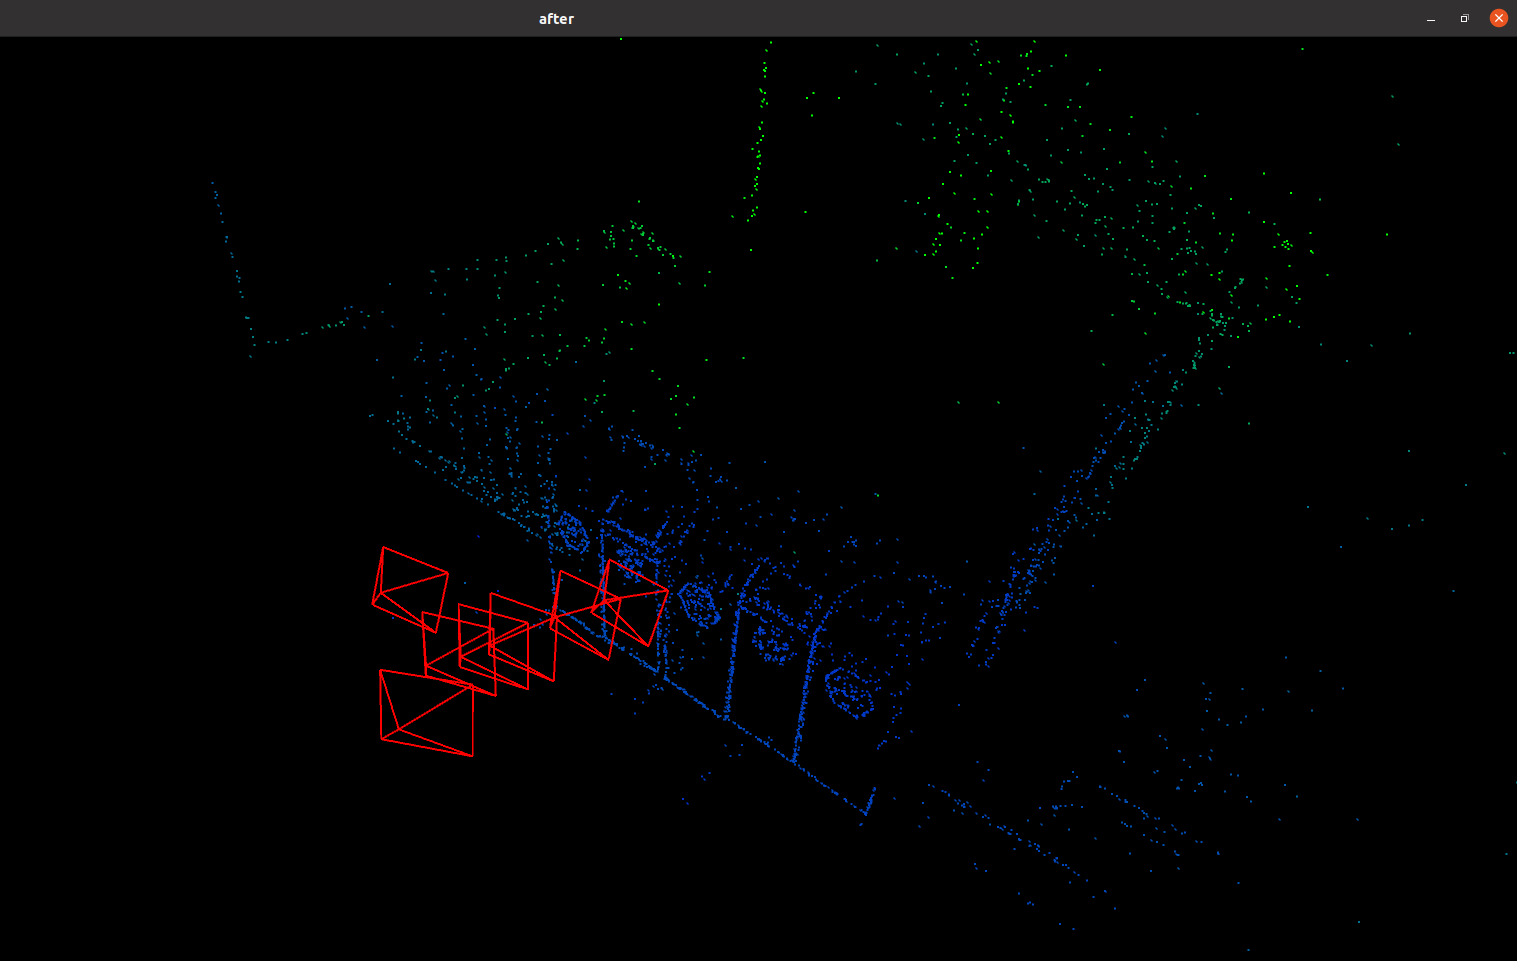
\includegraphics[width=4.8in]{ch7_3_2.png} {图3.2 g2o优化后的点云}
\end{figure}

实验了自己写的雅可比和让g2o自己写雅可比的性能对比,自己写的雅可比优化速度要快一些,且边的代价也要小一些,对比分别如图3.3和3.4所示:
\begin{figure}[H]
\centering
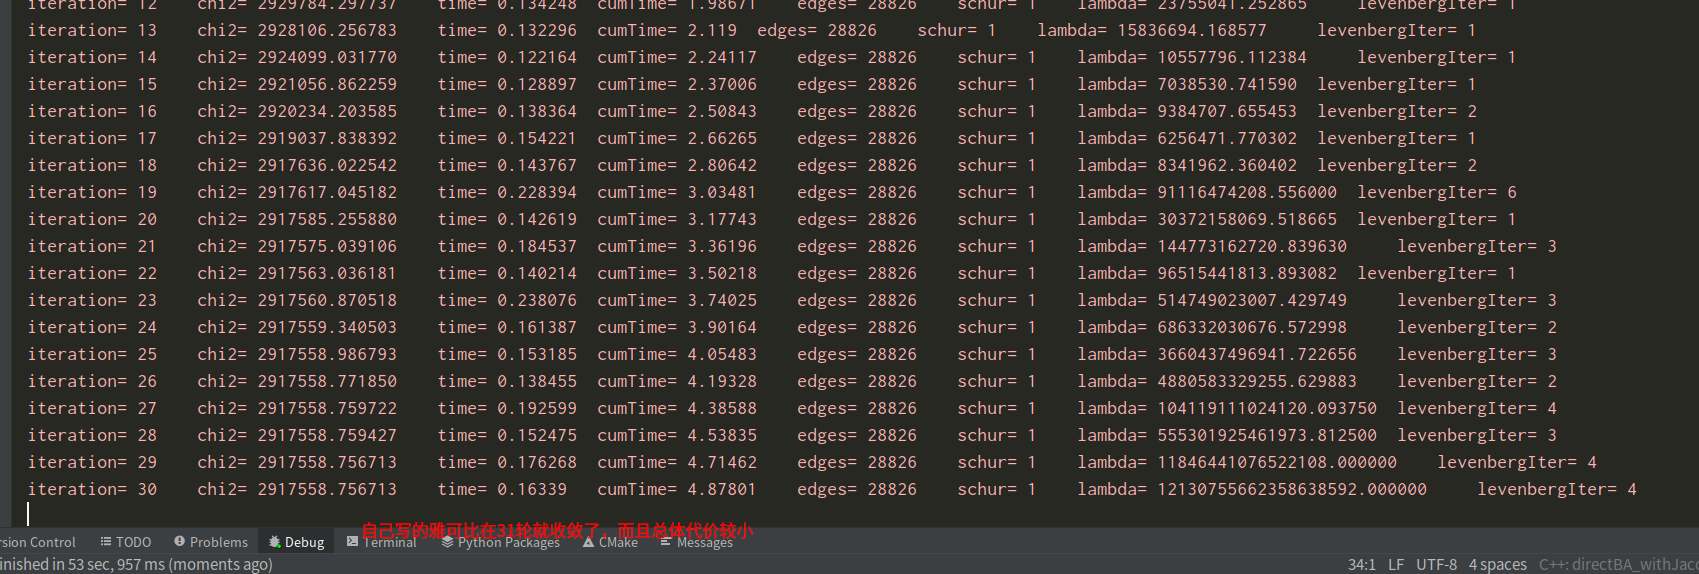
\includegraphics[width=4.8in]{ch7_3_3.png} {图3.3 自己实现雅可比的运行结果}
\end{figure}

\begin{figure}[H]
\centering
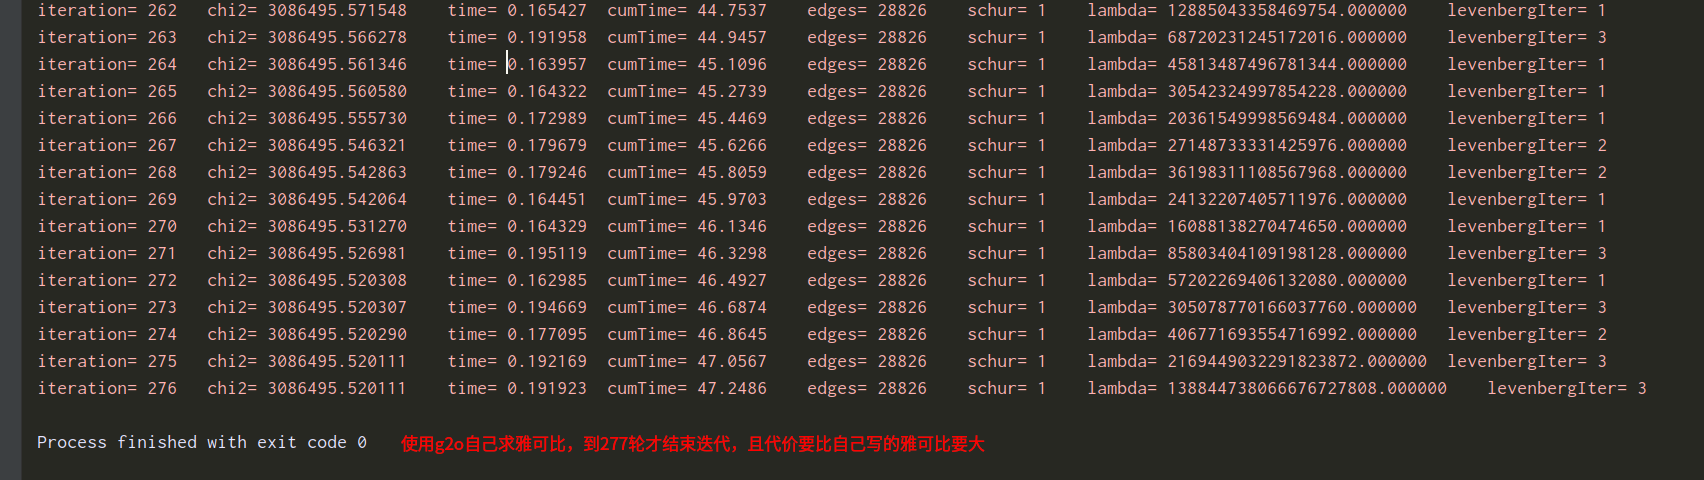
\includegraphics[width=4.8in]{ch7_3_4.png} {图3.4 g2o自动求雅可比的运行结果}
\end{figure}


\begin{thebibliography}{99}  
\bibitem{ref1}J. Engel, V. Koltun, and D. Cremers, “Direct sparse odometry,” arXiv preprint arXiv:1607.02565,
2016.

\bibitem{ref2}https://blog.csdn.net/qq\_37746927/article/details/123787617
\end{thebibliography}

\end{document}